\documentclass[twocolumn]{article}

\usepackage{lipsum} 
\usepackage{hyperref}
\usepackage{placeins}
%\hypersetup{colorlinks,urlcolor=blue}
\hypersetup{colorlinks,urlcolor=black}

\usepackage{graphicx}

\title{Habitat Connectivity Modelling with Spatial Absorbing Cell DEVS}
\author{Griffin Barrett}

\graphicspath{ {./images/} }

\begin{document}

\twocolumn[
\begin{@twocolumnfalse}
	\maketitle
	\begin{abstract}
		\begin{center}
		Quantifying landscape connectivity and animal movements in Cell-DEVS.
		\end{center}
	\end{abstract}
\end{@twocolumnfalse}
]
\clearpage
\section{Introduction}

Landscape connectivity is a very important measure of overall habitat quality (Taylor et al.
1993).
Unfortunately, accurately calculating landscape connectivity from available map data is no simple task (Fletcher et al. 2011, Sawyer et al. 2011).

Prominent models in the field of movement ecology broadly fall into two camps, simple convolution (Beyer, H. L. et al. 2019), and markov chains (Marx, A.J. et al. 2020). The former apply a variety of blur and filter algorithms to spatial datasets to get an overall picture of the quality of a landscape or to predict animal populations and movements. This has some success simply because of how fast it is, making large scale models with a simple ``more data points and more precision makes more accuracy" approach. The second camp use their more sophisticated and more formal models to make far more accurate predictions, at the cost of having a tight upper bound on the amount of data that they can consider at a time due to memory constraints. The memory footprint of fully connected adjacency matrixes grows with the square of the dataset and linearly with both the duration of the model and the precision of the data. This cruel reality keeps these models only considering a few square kilometres at a time.

This model attempts to toe the line between these two extremes, by having a model almost as sophisticated as the second camp, while keeping a linear space complexity with the size of them model.

\section{Background}

Cell-DEVS is a simulation formalism based on the DEVS family of simulation formalisms. It simplifies modelling cellular automata and specially structured models. It does this my having the concept of a neighbourhood to describe the connectedness of cells in the space, and the concept of a local computation to describe how a cell evolves over time. Communication between cells is simplified through the use of delays and the global advance function is simply running and updating all of the cells with pending local functions. This formalism simplifies the design of models that it is aligned with by handling much of the complexity of a general DEVS model, simplifies reading and modifying an existing model by giving modellers a common framework to work off of, and adds an element of portability by allowing any model to be implemented and run on any number of simulation engines.

\section{Definition and Implementation}

\subsection{High Level Description}

The area of interest is divided into equally sized square cells. Each of these cells are given a pair non-negative real values representing how easy it is to move through that cell and how likely an animal is to die if they spend a time step in that cell. Frome these values, scalars are calculated representing what proportion of the animals that start a time step in the cell end that time step in each of the 4 boarder cells, how many stay in place, and how many die. 

Once those values are cached, the local function is as follows.
\begin{enumerate}
	\item Increment the count of animals that died here.
	\item Sum the animals that will come here from neighbouring cells and that will stay here from this cell, and replace this cell's population with that sum.
\end{enumerate}
\subsubsection{Caveats}

Timestep 0 is used to pre-calculate the travel rate values. Each cell looks at it's neighbours' pre-calculated values and population with each of it's local computations, requiring that those values need to be there before any travel can happen. This is not a race condition or a crash risk with this implementation, but it is an inconvenience.

These cells have a very large state space of approximately $2^{64^{10}}$, of which $2^{62^{2}}$ are possible on any given run under normal circumstances. With the exception of boarder cells and cells with permeability of 0, they are not expected to pacivate during a normal run. This means that we are paying the full local computation for every cell, increasing the need for that computation to be simple and fast.

\subsection{Formal Description}

Formally, this model is defined as an Executable Synchronous Cellular Automata as follows:

\begin{verbatim}
ESCA = <S,n,{t1,,,tn},C,eta,N,B,T,tau,q.Z>
\end{verbatim}
\begin{verbatim}
S = {
  perm:{real >=0}, #permiability
  leth:{real >=0}, #lethality
  pop:{real >=0},  #population
  dead:{real >=0}, #deaths
  rate:{
    sparce map from 
    	{cell_position in N}
    	to 
    	{real >=0}
  }
}
\end{verbatim}
Real numbers are taken to be IEEE 754 double-precision floating-point numbers and therefore form a finite though very large alphabet.
\begin{verbatim}
n = 2
{row,col}
eta = 5
N = [(0,0), (0,1), (1,0), (0,-1), (-1,0)]
\end{verbatim}
\begin{verbatim}
Cells outside the space are taken to be
{0,0,0,0,{}}
and do not have their tau function called
\end{verbatim}
\begin{verbatim}
T : the emergent global transition function
\end{verbatim}
\begin{verbatim}
def tau(self, state, neighbors):
  if self.rate is empty:
    # Only ever at time step 0 
    total_perm = sum(
      n.perm for n in neighbors
    )
    if total_perm == 0:
      for n in neighbors:
        state.rate[n.position] = 0
    else:
      for n in neighbors:
        state.rate[n.position]=(
          (1-self.leth)*
          n.perm/total_perm
        )
  else:
    # Every time step after 0
    state.dead=(
      self.dead+self.leth*self.pop
    )
    state.population=(
      sum(
        n.rate[self.position]*n.pop
        for n in neighbors 
        if self.position in n.rate
      )
    )
\end{verbatim}
\begin{verbatim}
q.Z = {integer >= 0} =
 {0, 1, 2, 3,...}
\end{verbatim}

This ESCA is implemented in Cadmium Cell-DEVS with a time advance of $1$ and a non-premptive delay.

\section{Results}
\FloatBarrier
All of these runs start with $1.0\times$ the total population, concentrated in one cell. The scales on the right shows the proportion of the initial total population in each cell and the colour range is shifted to match the range of values at any given timestep.

A simple test scenario is to start with the entire population on the left, and provide two hallways that they can move through. This kind of test is used to see simple behaviours and acts as a sanity check for the model.

\begin{figure}[h!]
	\begin{center}
		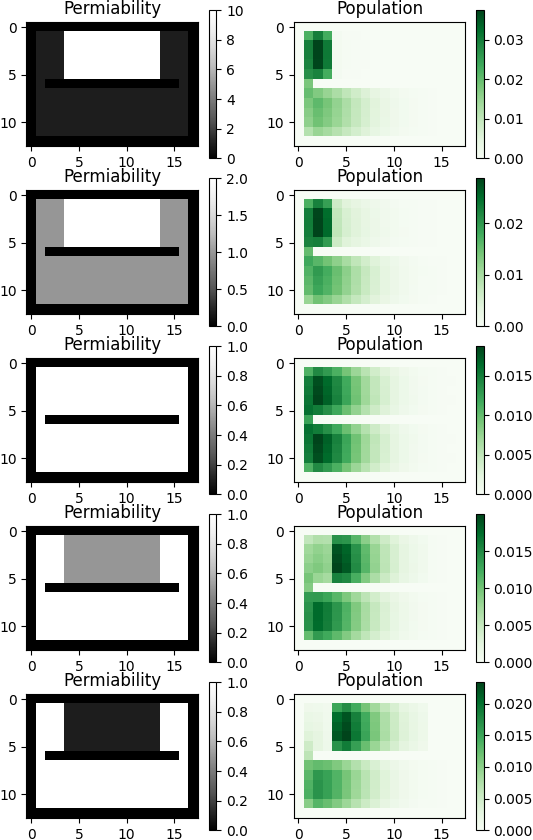
\includegraphics[width=18em]{halls_permeability.png}
		\caption{Animal spread through halls of permiabilitys \{0.1, 0.5, 1, 2, 10\}, at time 50}
		\label{fig:halls_permeability}
	\end{center}
\end{figure}

As we can see in figure \ref{fig:halls_permeability}, permiability is working sencibly.

This model also described lethality. The scale works in much the same way as population.

\begin{figure}[h!]
	\begin{center}
		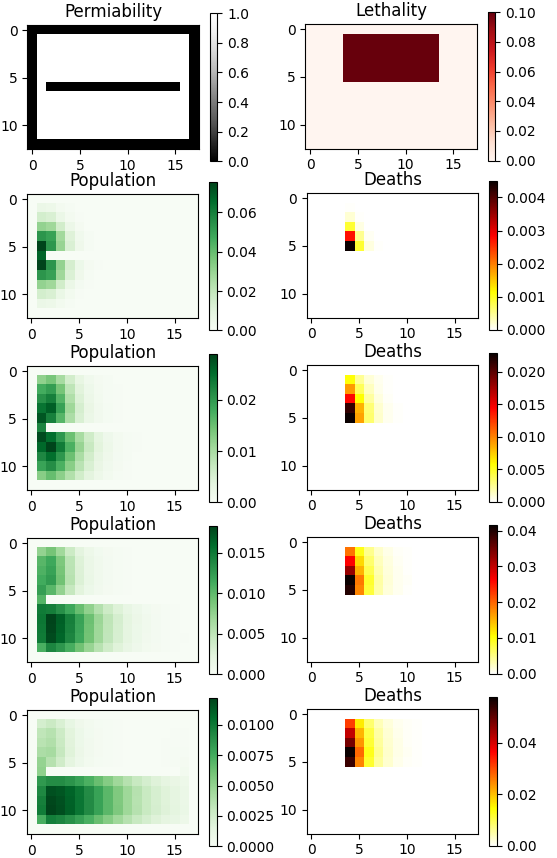
\includegraphics[width=18em]{halls_lethality_10.png}
		\caption{Animal spread through halls of lethality 0.1, at times \{10, 25, 50, 100\}}
		\label{fig:halls_lethality_10}
	\end{center}
\end{figure}

\begin{figure}[h!]
	\begin{center}
		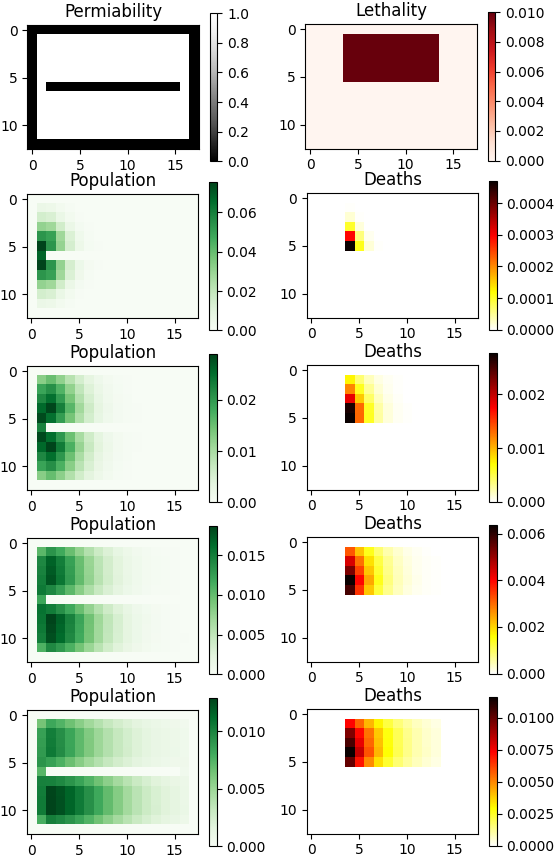
\includegraphics[width=18em]{halls_lethality_100.png}
		\caption{Animal spread through halls of lethality 0.01, at times \{10, 25, 50, 100\}}
		\label{fig:halls_lethality_100}
	\end{center}
\end{figure}

\begin{figure}[h!]
	\begin{center}
		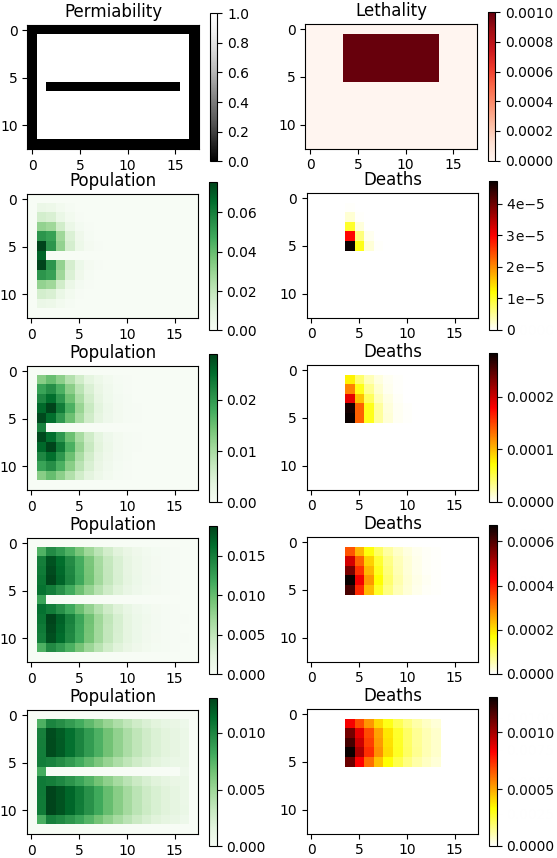
\includegraphics[width=18em]{halls_lethality_1000.png}
		\caption{Animal spread through halls of lethality 0.001, at times \{10, 25, 50, 100\}}
		\label{fig:halls_lethality_1000}
	\end{center}
\end{figure}

As figures \ref{fig:halls_lethality_10}, \ref{fig:halls_lethality_100}, and \ref{fig:halls_lethality_1000} show us, the more lethal the area, the fewer animals make it through, despite having the same permiability. This is what we would expect to see and is another point to the model giving sencable output.

Once the model is doing what it should be for these trivial examples, we can try it out on more complex scenarios to see what emergent behaviours we can find.

\begin{figure}[h!]
	\begin{center}
		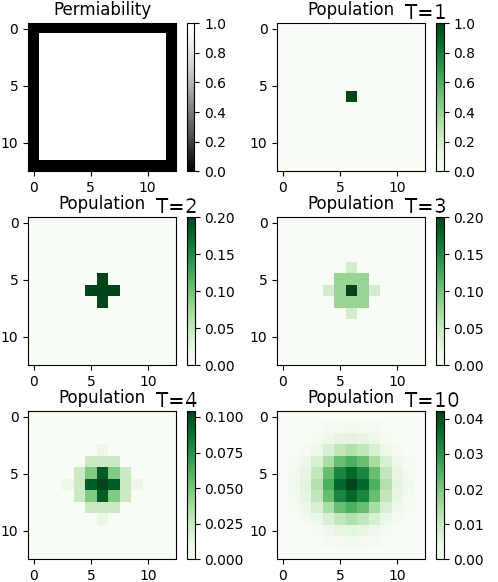
\includegraphics[width=18em]{small_flat_field.png}
		\caption{Animal spread on a small flat field, at times \{1, 2, 3, 4, 10\}}
		\label{fig:small_flat_field}
	\end{center}
\end{figure}

The kind of random walk that this model defaults to, where any animal is equally likely to go into any cell in it's neighbourhood aproximates a gausian. We can see this clearly in figure \ref{fig:small_flat_field} and is what we would expect to see. 

\begin{figure}[h!]
	\begin{center}
		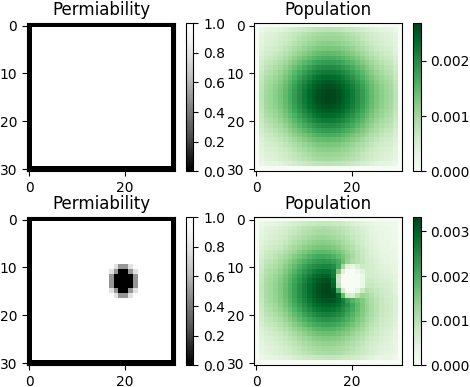
\includegraphics[width=18em]{flat_field_with_or_without_rock.png}
		\caption{Flat field with and without rock obstructing movement, at time 150}
		\label{fig:flat_field_with_or_without_rock}
	\end{center}
\end{figure}

In figure \ref{fig:flat_field_with_or_without_rock}, we can start to see more interesting paterns. Notice how the animals take longer to get behind the rock than it would otherwise take to the same spot directly? This is an early first sign that our model is more than just a convolution.

\begin{figure}[h!]
	\begin{center}
		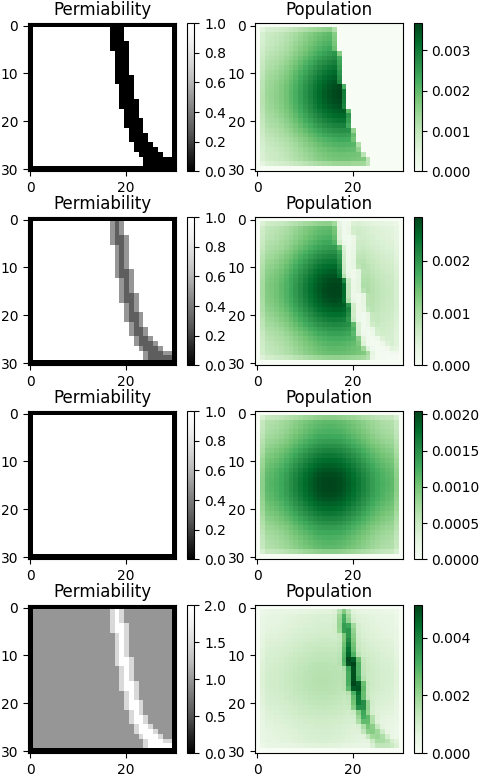
\includegraphics[width=18em]{river_and_friends.png}
		\caption{Flat field with various obstructions, at time 200}
		\label{fig:river_and_friends}
	\end{center}
\end{figure}

Anamals will tend to take lower effort paths like roads and paths to travel farther in the same amount of time. We see this in action in figure \ref{fig:river_and_friends}. With this, we would predict things like wolves haveing their teritory expand when and where logging roads are constructed, simply because they can move farther in a day. Something else that this predicts is that animal sightings on roads will be over estimates of the true wildlife population, because the ease of use makes the animals concentrate on or near the roads.

\begin{figure}[h!]
	\begin{center}
		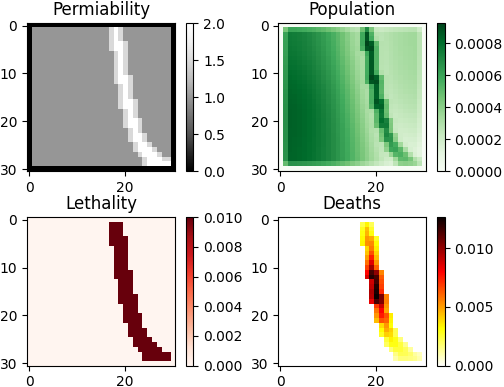
\includegraphics[width=18em]{active_road.png}
		\caption{Flat field with an active road, at time 450}
		\label{fig:active_road}
	\end{center}
\end{figure}

Roads do more than just allow animals to move, they also bring cars. Cars and trucks are often linked to an increaced death rate amung the local animal population. Animals in this model do not know to run from danger, and continue to use the road for it's convenience dispite the risks. This has the effect of causing a local decrease in animal population near the road, and is illistrated clearly in figure \ref{fig:active_road}.
\FloatBarrier
\section{Improvements}

The simulation frame is that no new animals are born, no animals interact with one another, there is only one kind of animal, and the landscape does not change over time. Each of these constraints can be a focus for improvements.

One area of improvement can come in the form of making permiability and lethality some function of population and a new set of local constants. This allows us to model animals spreading out deliberatly, or even congregating up to some population, by modulating permiability, and animals starving or breeding by modulating lethality and both alowing it to be negative and recording births seperatly from deaths. These two changes would make the animals behave less like an ideal gass and more like we expect life to behave. These changes would come at the cost of needing to recalculate rates every time step rather than only at time=0, which would have a potentially dramatic runtime impact.

The next area of improvement can come from having more than one population in each cell, or by having more than one layer each with their own population. This would let us model more than one kind of animal at a time, and if we combined this with the first round of improvements we can model preditor/prey dynamics and even symbiotic relationships. This would come at the cost of increasing memory footprint and yet more runtime complexity.

Another area of improvement can addres the unchanging nature of the landscape. The permiability and lethality of the landscape can be pulled off onto their own layer and alowed to evolve dynamicly, or they can can predetermined changes at set times, or even be fed their values from an extencive input file. This addition would allow us to model changing seasions in it's most simple incarnation. One step farther would be to allow the landscape to change in responce to the populations and deaths of the animals above it. Perhaps permiability goes up as the animals trample paths into the grass, and the dead fertalize the ground. This can even be done in conjunction with the first two areas of improvement to make what is quickly becoming a very sophisticated ecological model. This set of changes comes with a very similar set of costs as the first one, more recalculation and more runtime.

Another area of improvement is runtime and memory footprint. These are allways present, regardles of the model at hand, so they often do not bear repeating, but they are especially relevant here. These models are at their strongest and most usefull when they can comfertably handle $>$$10^{8}$ cells over $>$$10^{3}$ timesteps, which is no small feat. Additional steps that can be taken to speed up the simulation should not be overlooked, even if they reduce the sophistication of the model further. Perhaps we can look into discounting any animals that stay in the same cell and instead mandate that they all move, decreasing computation by a factor of $1/6$, or perhaps we can have animals only move north/south on even time steps, and east/west on odd steps, further redusing the per-step computation and the comunication between cells. These changes would decrease presition, but that may be worth the cost if the speedup is remarkable enough.

\section{Conclusion}

This model effectively implements modern ecological connectivity techniques using the Cell-DEVS formalism. This model demonstrates the emergent behaviour present is other sophisticated models, and is relatively simple and straightforward to understand and work with. 

See \url{https://github.com/xlirate/Cadmin-Cell-DEVS-SAMC} for the code.

\section{Future Work}

With this implementation as a prototype, a double buffered paralelized implementation is in the works, with the hopes of being able to run on national or international sized datasets on consumer hardware. 

\section{Bibliography}

\begin{itemize}

\item Taylor, P. D. et al. 1993. Connectivity is a vital element of landscape
structure. – Oikos 68: 571–573. \url{
	https://doi.org/10.2307/3544927 }

\item Fletcher Jr., R. J. et al. 2011. Social network models predict movement and connectivity in ecological landscapes. – Proc. Natl
Acad. Sci. USA 108: 19282–19287. \url{https://doi.org/10.1073/pnas.1107549108}

\item Sawyer, S. C. et al. 2011. Placing linkages among fragmented habitats: do least-cost models reflect how animals use landscapes?
– J. Appl. Ecol. 48: 668–678. \url{https://doi.org/10.1111/j.1365-2664.2011.01970.x}

\item Beyer, H. L. et al. 2019. Substantial losses in ecoregion intactness highlights urgency of globally coordinated action. – Conservation Letters. 2020; 13:e12692. \url{https://doi.org/10.1111/conl.12692}

\item Marx, A.J. et al. 2020. samc: an R package for connectivity modeling with spatial absorbing Markov chains. – Ecography, 43: 518-527. \url{https://doi.org/10.1111/ecog.04891}

\end{itemize}

\end{document}








